\documentclass[11pt]{article}

%%%%%%%%%%%%%%Include Packages%%%%%%%%%%%%%%%%%%%%%%%%%%
\usepackage{xcolor}
\usepackage{mathtools}
\usepackage[a4paper, total={6in, 8in}, margin=1.25in]{geometry}
\usepackage{amsmath}
\usepackage{amssymb}
\usepackage{paralist}
\usepackage{rsfso}
\usepackage{amsthm}
\usepackage{wasysym}
\usepackage[inline]{enumitem}   
\usepackage{hyperref}
\usepackage{tocloft}
\usepackage{titlesec}
\usepackage{colortbl}
%%%%%%%%%%%%%%%%%%%%%%%%%%%%%%%%%%%%%%%%%%%%%%%%%%%%%%%%



\begin{document}
\Large \noindent \textbf{Physics 5C Discussion (Week 1)}\\
\normalsize
Department of Physics and Astronomy, UCLA\\

\noindent TA: Jinyan Miao (jnmiu@ucla.edu)\\
Office hours: Thursday 10-11 AM $\&$ 1-2 PM at PAB 2-429\\
Tutoring center hours: Friday 2-3 PM at PAB 2-429 (Zoom room also available)\\
\noindent\rule{8cm}{0.4pt}\\

\noindent\textbf{Problem 1:} In this class, vectors are generally considered as three-dimensional objects, that is, they have three independent components, denoted as $\vec{V}= (x,y,z) = x\,\hat{\i} + y\, \hat{\j} + z\,\hat{\text{k}}$. Here we consider three vectors $\vec{B}=1\,\hat{\j}$, $\vec{C} = 2\, \hat{\i}$, and $\vec{D} = 1\,\hat{\j} + 2 \,\hat{\i}$. \\

\noindent\textbf{Part (a)}: Find the length and the direction of the vector $\vec{D}$. Write its direction in terms of the angle it makes with respect to the $x$-axis of the coordinate system. \footnote{Hint: Use $\arctan$ and $\sqrt{?^2 + ?^2}$.}\\

\noindent\textbf{Part (b)}: Compute the dot products $\vec{B} \cdot \vec{C}$ and $\vec{C} \cdot \vec{D}$, using whatever method you like.\\

\noindent\textbf{Part (c)}: Find the direction of the cross product $\vec{B}\times \vec{C}$, and the direction of $\vec{B}\times \vec{D}$. \footnote{Hint: Both $\vec{B}\times \vec{C}$ and $\vec{B} \times \vec{D}$ should be parallel to some axis in the coordinate system, so you don't need to compute any angle to describe the direction of the vectors.}\\

\noindent\textbf{Part (d)}: Find the direction of $\vec{C}\times \vec{B}$. How does it compare to the direction of $\vec{B}\times \vec{C}$? \\

\vspace*{7cm}
\begin{center}
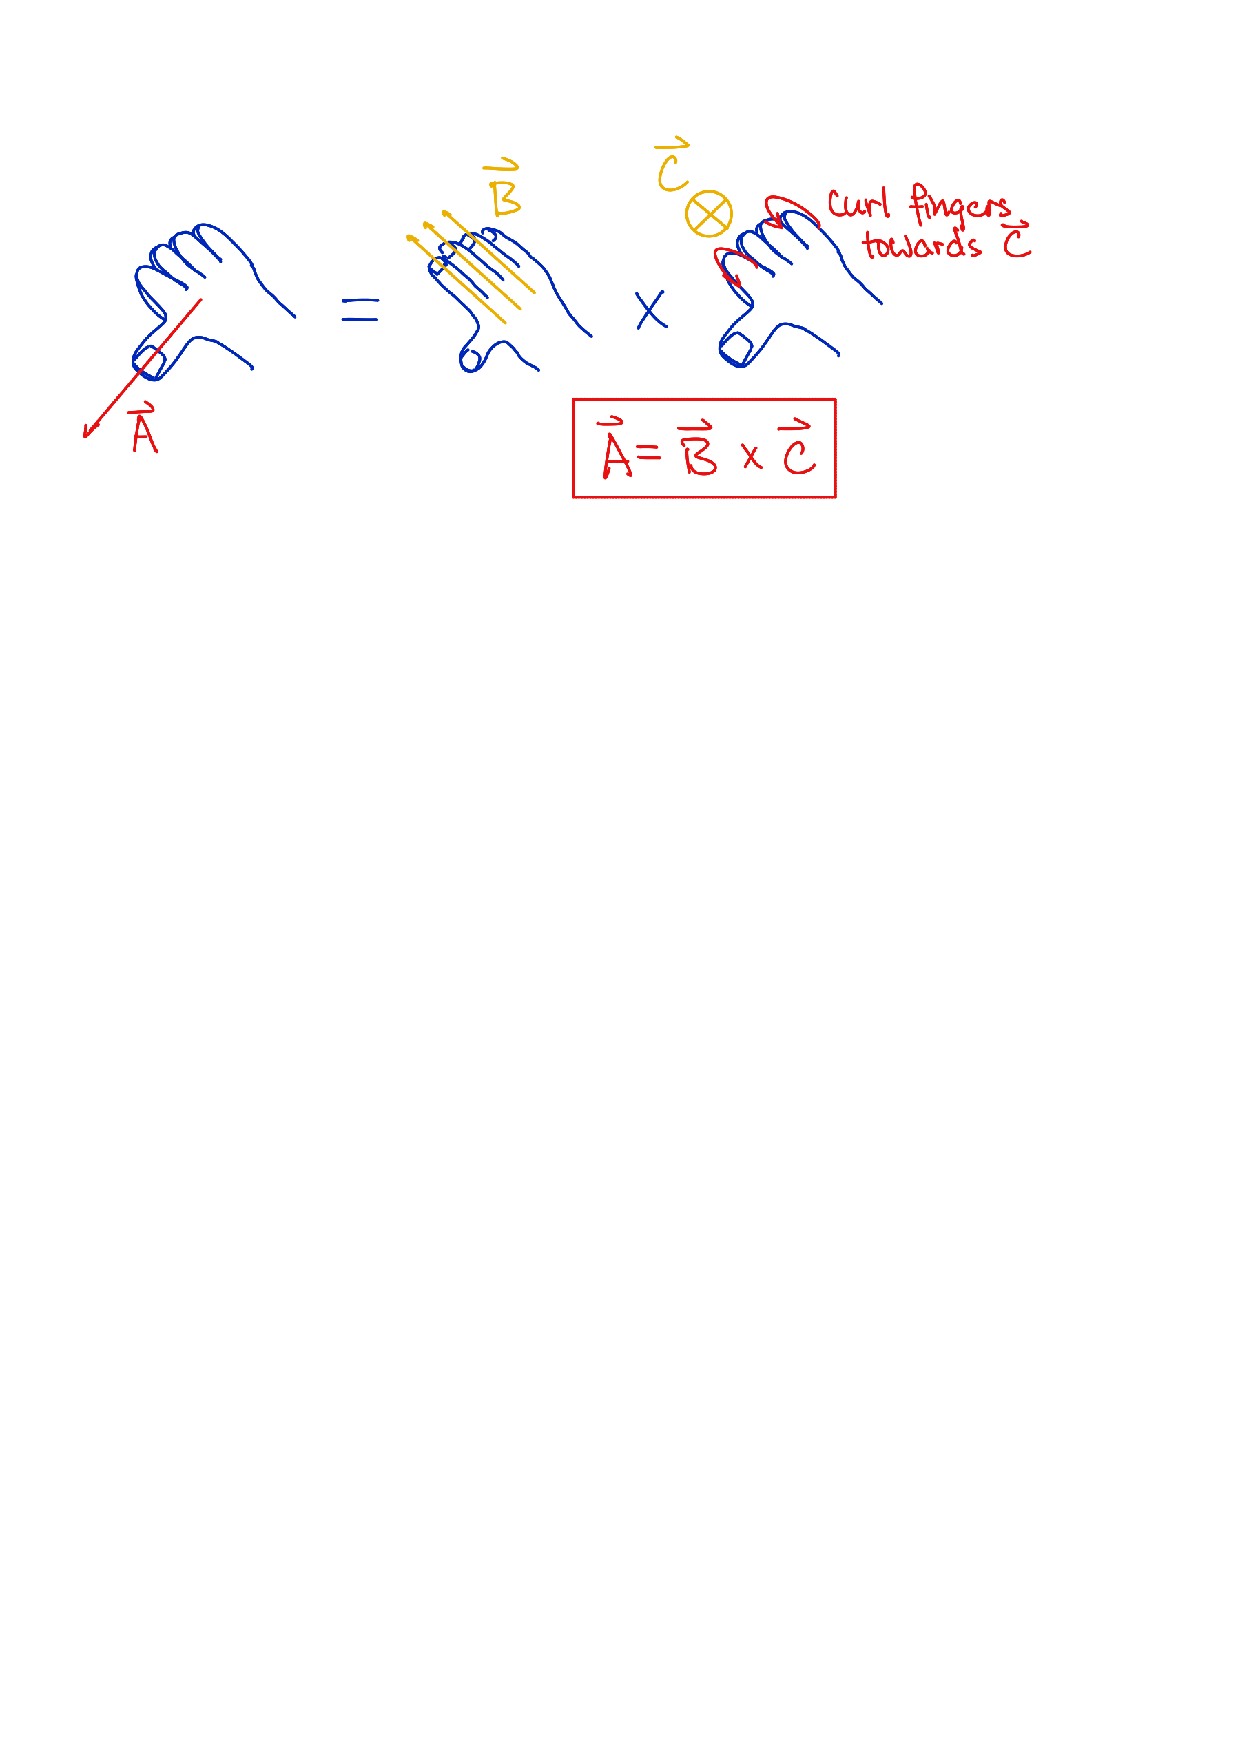
\includegraphics[scale=0.65]{rhr}
\end{center}

\newpage
\noindent\textbf{Problem 2:} Jinyan in a high-tech metallic spacesuit is being attracted by two gigantic magnets. Neglect gravity and friction in this problem. The magnetic forces he experiences are $F_1 = 1000$\,N to the left (due to the magnet on the left) and $F_2 = 100$\,N downwards (due to the magnet at the bottom). The mass of Jinyan with the spacesuit is 100\,kg. Assume that he is initially at rest at the origin, and the forces that he experiences stay constant throughout his journey. Where can you find Jinyan after $t$ seconds? Express your final answer as a position vector in terms of $t$. \footnote{Hint: Newton said $\vec{F}_{\text{net}} = m\vec{a}$.}\,\footnote{The kinematic equation for a constant acceleration $a_y$ in the $y$-direction is $$y =\frac{1}{2} a_yt^2 + v_{0,y}t + y_0\,.$$}
\begin{center}
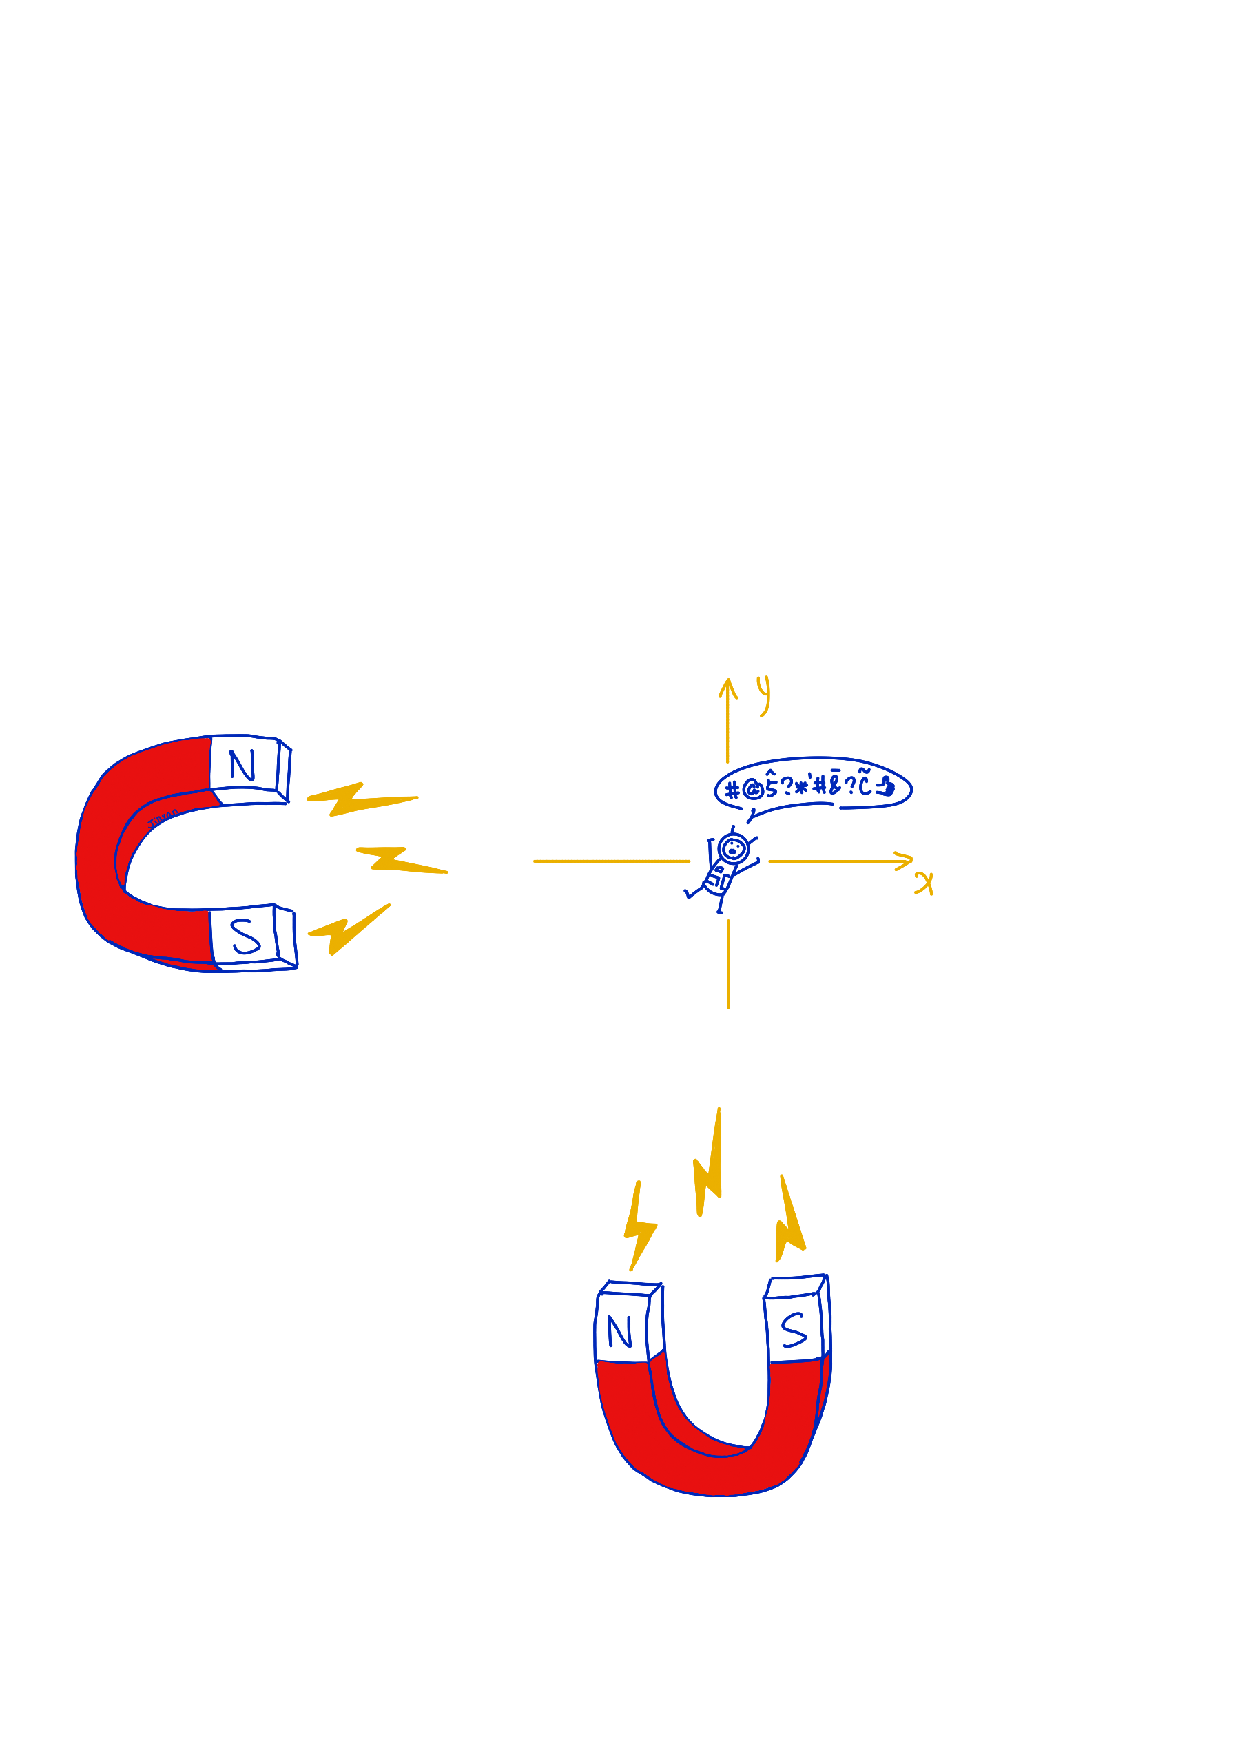
\includegraphics[scale=0.65]{magnet}
\end{center}


\newpage
\section*{Problem 1}
(a) The length of $\vec{D}$ is 
\begin{align*}
D =\sqrt{2^2 +1^2} = \sqrt{5}\,.
\end{align*}
The angle $\theta$ that $\vec{D}$ is making with respect to the $x$-axis is
\begin{align*}
\theta = \arctan\left(\frac{1}{2}\right) = 26.6^\circ\,.
\end{align*}
Note that if $\vec{D}$ has a nonzero $z$-component, then we should use $D = \sqrt{x^2 + y^2 + z^2}$ to calculate its length.\\

\noindent (b) Straightforward computation, 
\begin{align*}
\vec{B}\cdot \vec{C} = 0 \cdot 2 + 1 \cdot 0 = 0\,,\qquad 
\vec{C}\cdot \vec{D} = 2\cdot 2 + 0 \cdot 1 = 4\,.
\end{align*}
For dot product, you multiply component-wise then add the components, the result should be a \textbf{scalar}.\\

\noindent (c) Using your right hand, with the right-hand rule, you should find that the direction of $\vec{B}\times \vec{C}$ is pointing into the page (negative $z$-direction). The direction of $\vec{B}\times \vec{D}$ is also pointing into the page (negative $z$-direction). Notice that cross product gives a \textbf{vector}, not a scalar.\\

\noindent[\textbf{UPDATED}] Some of you asked about the numerical computation of the cross product. I can do it here using $\vec{B}$, $\vec{C}$, and $\vec{D}$ as an example. First I need to write them as three-dimensional vectors. $\vec{B} = (0,1,0)$, $\vec{C} = (2,0,0)$, and $\vec{D} = (2,1,0)$. Then using the formula for cross product, 
\begin{align*}
\vec{B}\times \vec{C} = \left(
B_yC_z - C_yB_z\,,\
B_zC_x - C_zB_x\,,\
B_xC_y - C_xB_y
\right) = (0,\,0,\,-2)\,.
\end{align*}
This is indeed pointing in the negative $z$-direction, which is defined as into the page.
\begin{align*}
\vec{B}\times \vec{D} = \left(
B_yD_z - D_yB_z\,,\
B_zD_x - D_zB_x\,,\
B_xD_y - D_xB_y
\right) = (0,\,0,\,-2)\,.
\end{align*}
Same result as $\vec{B}\times \vec{C}$. These two turn out to have the same result because the cross product indicates ``how much of one vector is perpendicular to the other one." (the more precise physical meaning or geometrical meaning of cross product is more complicated though ... you can try to Google it for a better explanation) The portion of $\vec{D}$ that is being perpendicular to $\vec{B}$ is actually $\vec{C}$. Therefore $\vec{B}\times \vec{C} = \vec{B}\times \vec{D}$.\\

\noindent (d) Right-hand rule again, $\vec{C}\times \vec{B}$ points out of the page (positive $z$-direction). This is the negative of $\vec{B}\times \vec{C}$. Mathematically, this is
\begin{align*}
\vec{C}\times \vec{B} = \left(
C_yB_z - B_yC_z\,,\
C_zB_x - B_zC_x\,,\
C_xB_y - B_xC_y
\right) = (0,\,0,\,2)\,.
\end{align*}
Here we have a very general rule for cross product of vectors $\vec{v}$ and $\vec{u}$
\begin{align*}
\vec{v}\times \vec{u} = -\vec{u}\times \vec{v}\,.
\end{align*}
However, for dot product, 
\begin{align*}
\vec{v}\cdot\vec{u} = \vec{u}\cdot \vec{v}\,.
\end{align*}

\section*{Problem 2}
The net force that Jinyan experiences is 
\begin{align*}
\vec{F}_{\text{net}} = \vec{F}_1 + \vec{F}_2 = (-1000,\ -100) \,\text{N}\,.
\end{align*}
Notice here, we add the forces component-wise, and they have directions (to the left is negative in the $x$-direction, and downwards is negative in the $y$-direction, hence the negative signs). \underline{Never mix the $x$- and $y$-components, they should be treated independently}.\\

Now using Newton's second law, 
\begin{align*}
\vec{a} = \frac{\vec{F}_{\text{net}}}{m}= \left(-\frac{1000}{100}, \frac{-100}{100}\right) \,\text{m/s}^2 = (-10, -1) \,\text{m/s}^2\,.
\end{align*}
We see that $\vec{a}$ is a constant because $\vec{F}_{\text{net}}$ is a constant (in the problem we say the forces are constant throughout my journey). Therefore we can apply the kinematic equations (which require constant acceleration) for describing my motion in space. We have $a_x = -10$\,m/s$^2$ and $a_y = -1$\,m/s$^2$ as we just computed. The problem says I start at rest, thus $v_{0,x} = v_{0,y} = 0$\,m/s. Since I start at the origin, so $x_0 = y_0 = 0$\,m. Assembling everything, 
\begin{align*}
y = \frac{1}{2}a_y t^2 + v_{0,y} t + y_0 = -0.5 t^2 \,,\qquad
x = \frac{1}{2}a_x t^2 + v_{0,x} t + x_0 = -5 t^2 \,.
\end{align*}
Therefore, my position vector after $t$ seconds is 
\begin{align*}
\vec{x} = (-5 t^2,\ -0.5 t^2)\,.
\end{align*}

\hfill\break
I went to Chicago during the spring break ... Seems better than LA ...
\begin{center}
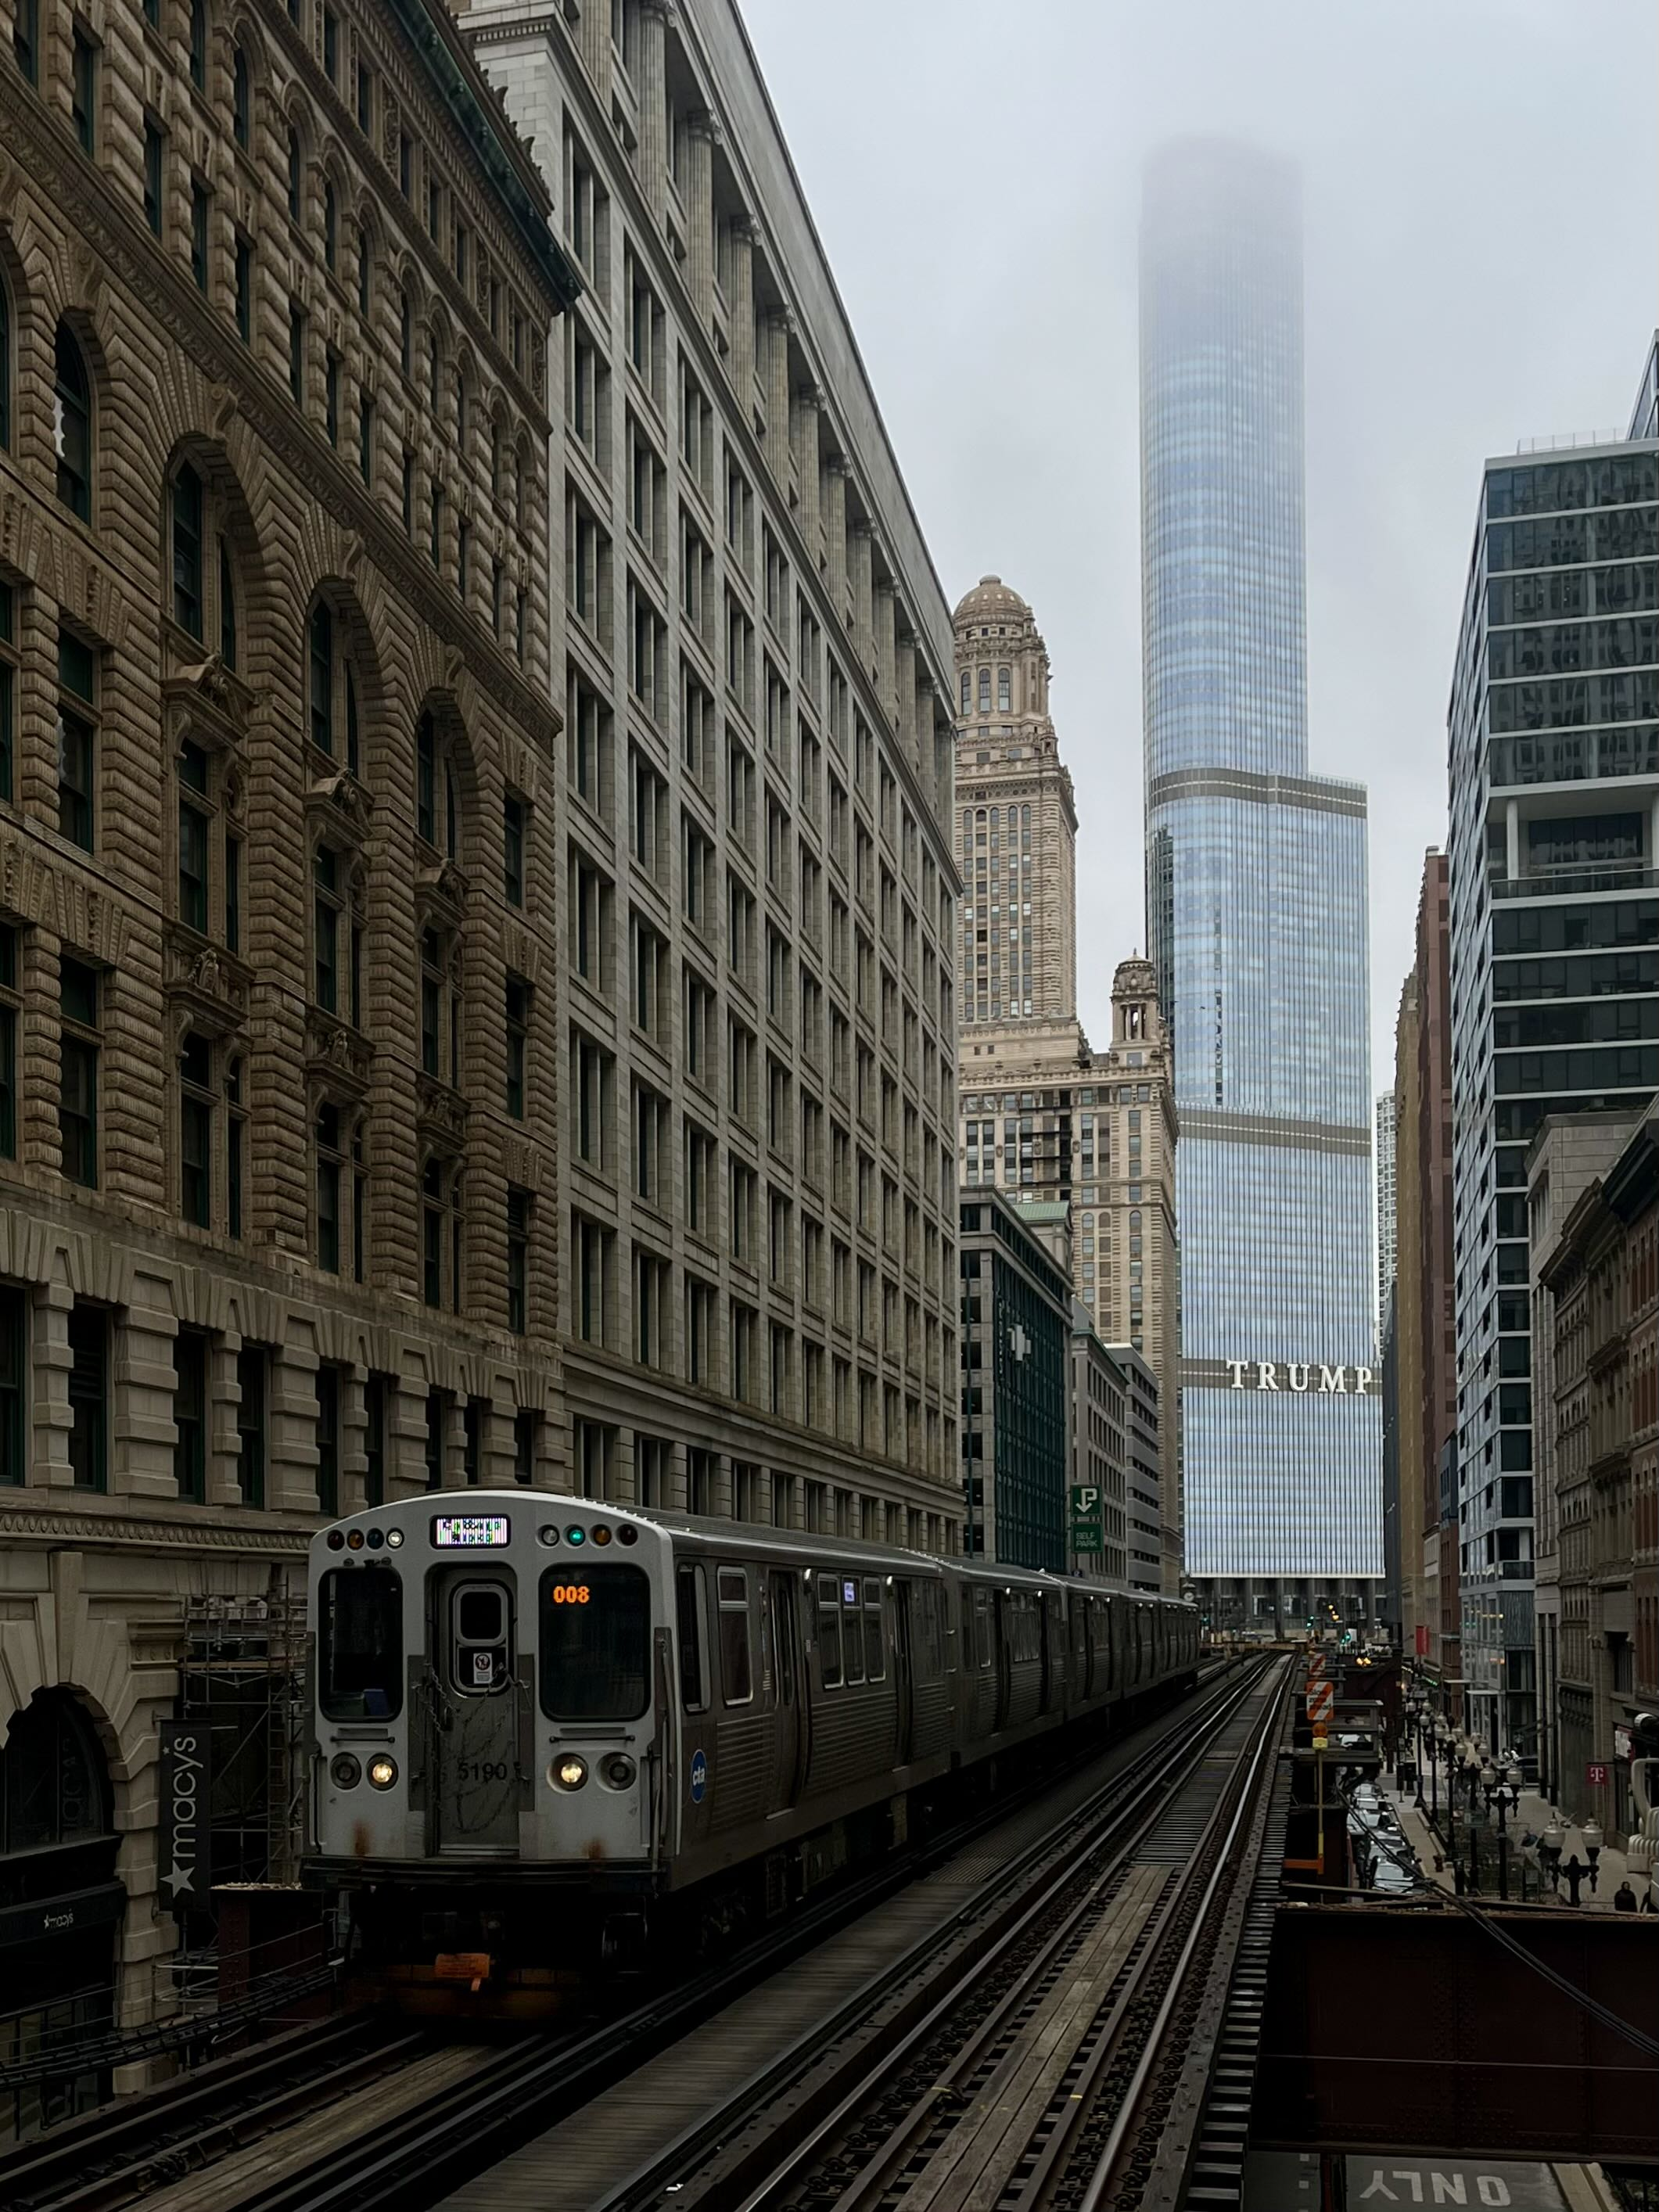
\includegraphics[scale=0.1]{IMG_1510.jpg}
\end{center}

\end{document}


